\documentclass[aspectratio=169,11pt]{beamer}
\usetheme{default}
\usecolortheme{default}
\setbeamertemplate{navigation symbols}{}

\usepackage[T1]{fontenc}
\usepackage[utf8]{inputenc}
\usepackage[french]{babel}
\usepackage{graphicx}
\usepackage{booktabs}
\usepackage{amsmath}
\graphicspath{{figures/}}

\setbeamercolor{frametitle}{fg=white,bg=blue!55!black}
\setbeamercolor{block title}{bg=blue!12!white,fg=blue!60!black}
\setbeamercolor{alerted text}{fg=red!70!black}

\begin{document}

\begin{frame}[t]{Avancement : optimisation du planning de bloc operatoire}
  \scriptsize
  \begin{columns}[T]
    % ------------------------------------------------------------------
    % Colonne gauche : ce qui a ete fait
    % ------------------------------------------------------------------
    \begin{column}{0.47\textwidth}
      \begin{block}{Realise}
        \begin{itemize}\itemsep1pt
          \item 10 methodes : 5 d'origine, 3 hybrides, 2 SMA Mesa.
          \item Affectation patients $\rightarrow$ vacations, cout a
                3 termes, budget temps.
          \item Benchmark 20 graines sur 3 echelles : 7, 300, 582 patients.
          \item 130 tests ; les 10 methodes atteignent l'optimum exact en
                petite instance.
          \item Re-planification dynamique (\texttt{hospital\_sim}), GUI,
                CLI.
        \end{itemize}
      \end{block}
      \begin{alertblock}{Resultats}
        Recuit simule et tabou$\times$recuit dominent (ecart moyen
        $<0{,}02$ sur $\sim$38\,800). ACO et genetique decrochent sur les
        donnees reelles.
      \end{alertblock}
    \end{column}
    % ------------------------------------------------------------------
    % Colonne droite : deux figures de resultats
    % ------------------------------------------------------------------
    \begin{column}{0.5\textwidth}
      \centering
      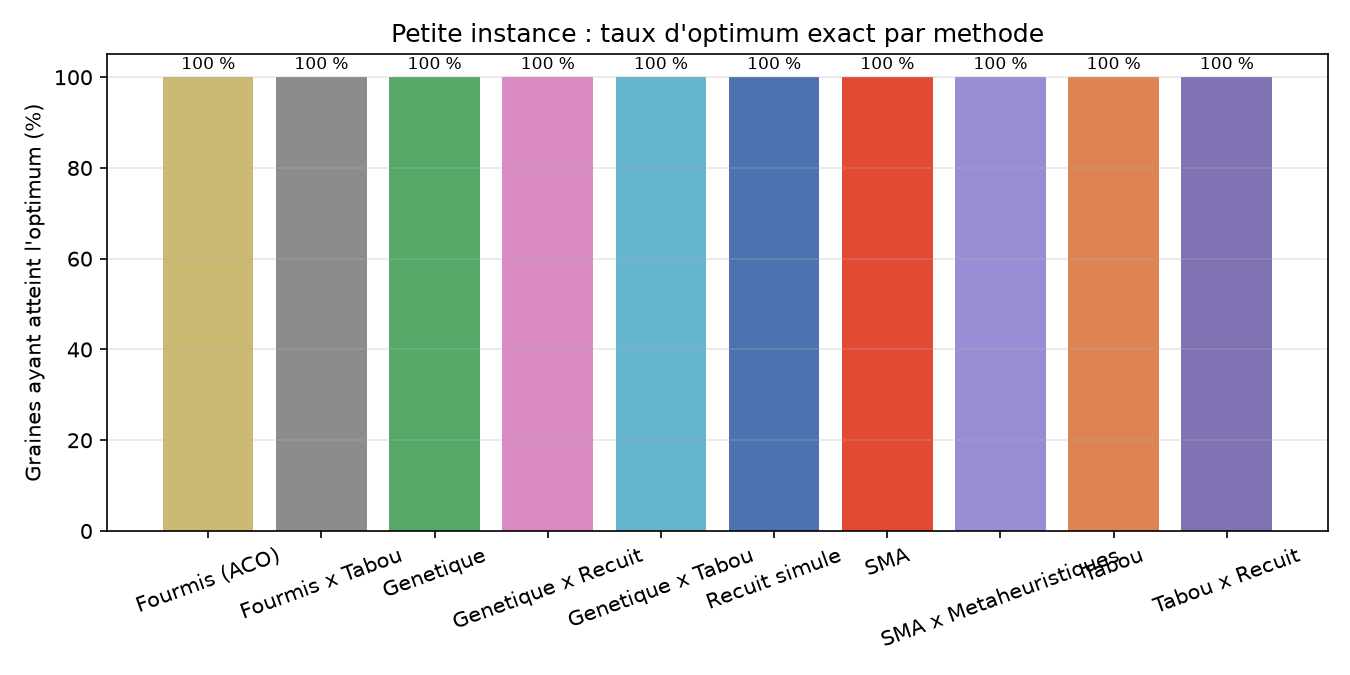
\includegraphics[width=\linewidth,height=0.30\textheight,keepaspectratio]{petite_taux_optimum.png}\\[1pt]
      {\tiny\color{blue!55!black}\textbf{Petite echelle :}
       10/10 methodes a l'optimum exact (20 graines).}\\[5pt]
      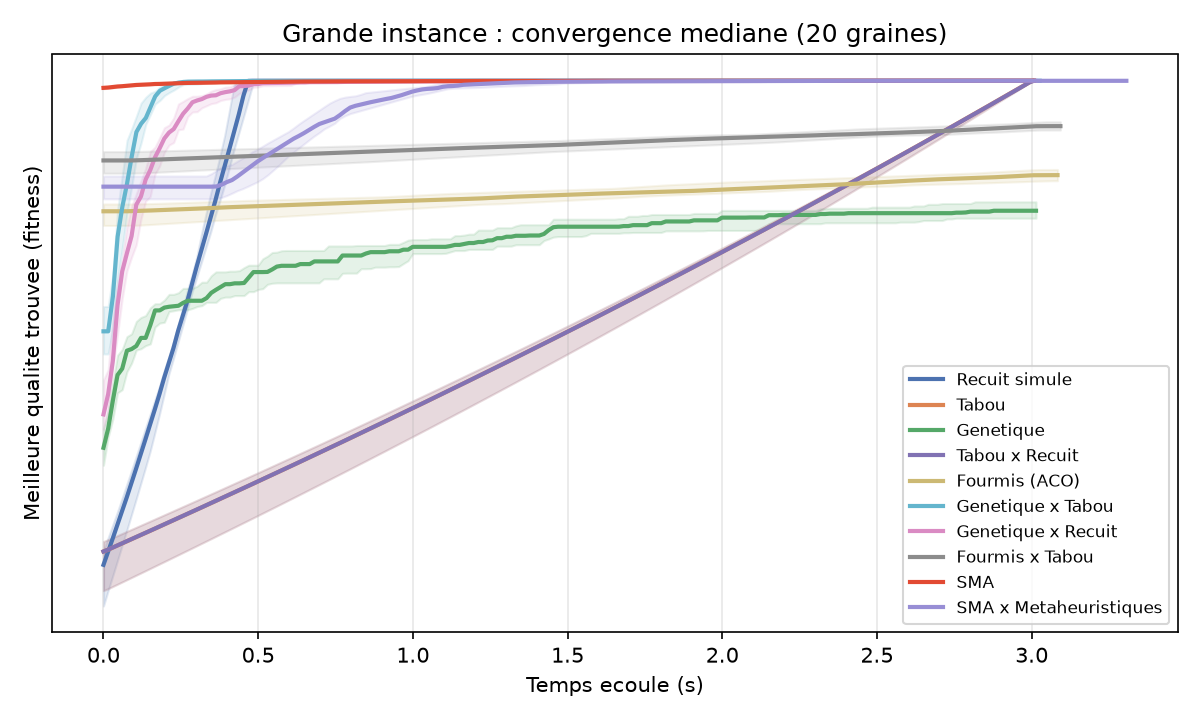
\includegraphics[width=\linewidth,height=0.30\textheight,keepaspectratio]{grande_convergence.png}\\[1pt]
      {\tiny\color{blue!55!black}\textbf{Grande echelle :}
       convergence a budget egal (300 patients, 3\,s).}
    \end{column}
  \end{columns}
\end{frame}

% =============================================================================
% Slide interface : API + application web
% =============================================================================
\begin{frame}[t]{Interface : API et application web}
  \scriptsize
  \begin{center}
    Une API \textbf{FastAPI} et une interface web : inscription et connexion.
  \end{center}
  \vspace{2pt}
  \begin{columns}[T]
    \begin{column}{0.5\textwidth}\centering
      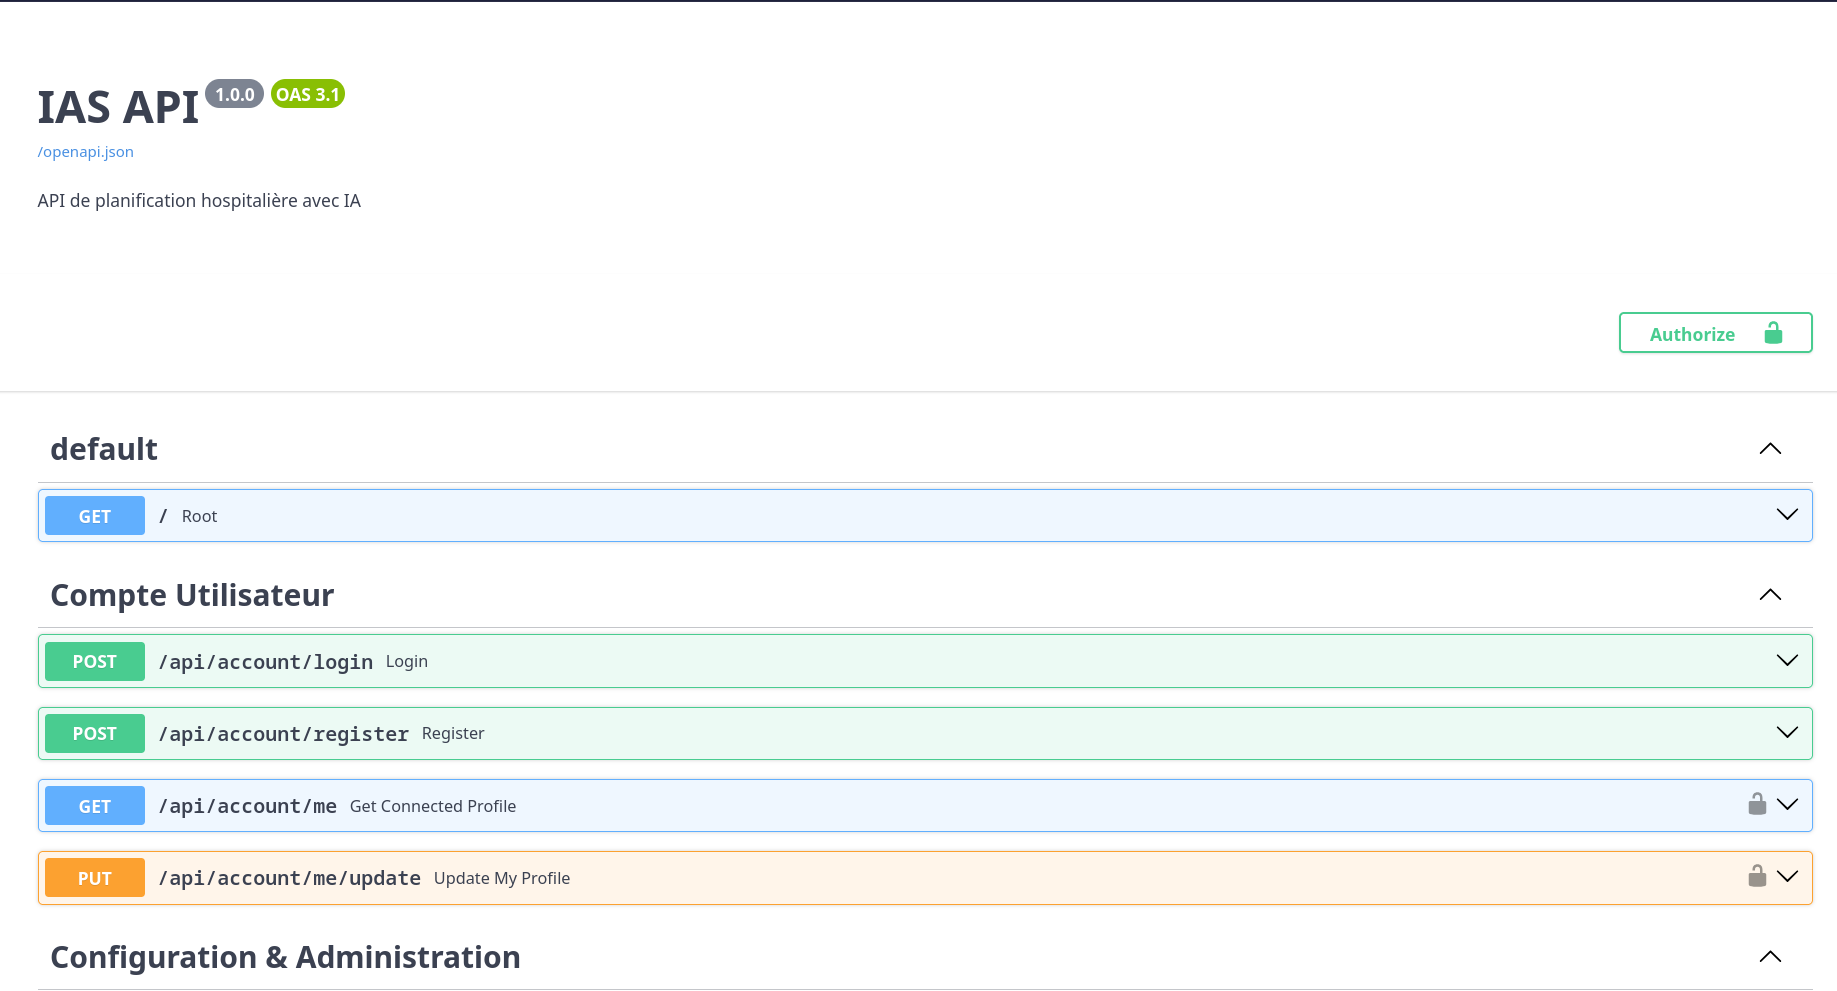
\includegraphics[height=0.40\textheight,keepaspectratio]{screen_API.png}\\[1pt]
      {\tiny API \texttt{IAS API} (Swagger)}
    \end{column}
    \begin{column}{0.25\textwidth}\centering
      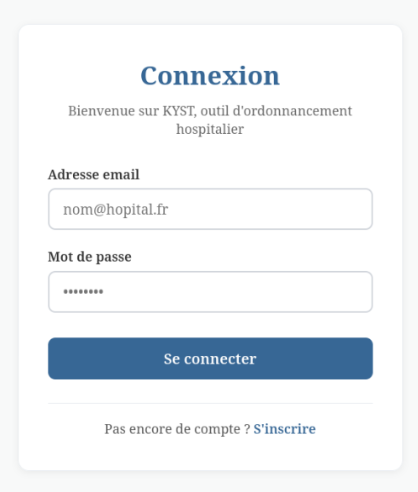
\includegraphics[height=0.40\textheight,keepaspectratio]{capture_interface_connexion.png}\\[1pt]
      {\tiny Connexion}
    \end{column}
    \begin{column}{0.25\textwidth}\centering
      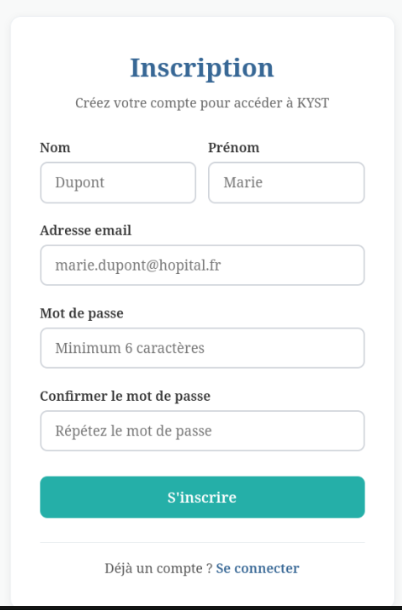
\includegraphics[height=0.40\textheight,keepaspectratio]{capture_interface_inscription.png}\\[1pt]
      {\tiny Inscription}
    \end{column}
  \end{columns}
\end{frame}

% =============================================================================
% Slide Machine Learning
% =============================================================================
\begin{frame}{Machine Learning : prédiction et planification robuste}

\vspace{-0.45cm}

\begin{columns}[T,onlytextwidth]

% ============================================================
% 1. PREDICTION
% ============================================================
\begin{column}{0.31\textwidth}

\begin{block}{1. Prédire les besoins des patients}
\scriptsize

\textbf{Performance vs. baselines simples}

\vspace{0.18cm}

{\Large\color{mcmPrimary}\textbf{-47.2\%}}\\
\textbf{MAE -- durée au bloc}\\
29.1 $\rightarrow$ 15.4 min

\vspace{0.2cm}

{\Large\color{mcmPrimary}\textbf{-60.2\%}}\\
\textbf{MAE -- durée de séjour}\\
1.107 $\rightarrow$ 0.441 jours

\vspace{0.25cm}

{\Large\color{mcmPrimary}\textbf{F1 = 0.922}}\\
\textbf{Type de prise en charge}\\
hospitalisation vs. ambulatoire

\vspace{0.30cm}

\textit{Évaluation sur patients hors entraînement}

\end{block}

\end{column}


% ============================================================
% 2. PLANIFICATION
% ============================================================
\begin{column}{0.34\textwidth}

\begin{block}{2. Améliorer la planification}
\scriptsize

\textbf{Prédictions ML intégrées à l'optimiseur}

\vspace{0.18cm}

{\Large\color{mcmPrimary}\textbf{21.8--27.0\%}}\\
\textbf{de réduction de l'objectif}\\
sur les grandes instances

\vspace{0.25cm}

\textbf{Gains par ressource}

\vspace{0.12cm}

Lits
\hfill
{\color{mcmPrimary}\textbf{33.9--37.4\%}}

\vspace{0.10cm}

Places ambulatoires
\hfill
{\color{mcmPrimary}\textbf{40.5--48.8\%}}

\vspace{0.30cm}

\textit{Compromis : critère bloc légèrement dégradé
($-3.2\%$ à $-9.0\%$)}

\end{block}

\end{column}


% ============================================================
% 3. ROBUSTESSE
% ============================================================
\begin{column}{0.31\textwidth}

\begin{block}{3. Tester l'incertitude sur le LOS}
\scriptsize

\textbf{Incertitude sur la durée de séjour}

\vspace{0.18cm}

{\Large\color{mcmPrimary}\textbf{\pm 1.02 jours}}\\
\textbf{Intervalle conforme à 90\%}

\vspace{0.12cm}

MAE = \textbf{0.412 jour}
\qquad
$R^2 = \textbf{0.789}$

\vspace{0.30cm}

\textbf{Sensibilité au LOS stochastique}

\vspace{0.15cm}

SA / Tabu / Hybride
\hfill
{\color{mcmPrimary}\textbf{\leq 1.2\%}}

\vspace{0.10cm}

ACO
\hfill
{\color{mcmPrimary}\textbf{0.1\%}}

\vspace{0.10cm}

GA
\hfill
{\color{mcmPrimary}\textbf{4.2\%}}

\vspace{0.30cm}

\textit{Incertitude propagée dans l'optimiseur}

\end{block}

\end{column}

\end{columns}
\end{frame}

\end{document}
